\chapter{Feature Extraction}
\label{ch:Feature Extraction}

\section{Conic Extraction}
In order to extract the conic $C$:
\begin{enumerate}
    \item Crop the image to the desired portion
    \begin{figure}[H]
    \centering
    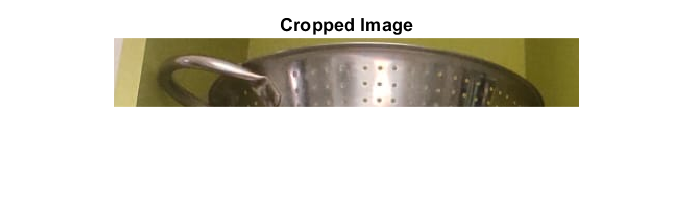
\includegraphics[height=9.5cm, width=\textwidth, keepaspectratio]{Report/Images/Features/Conic/CroppedImage.png}
    \caption{\label{fig:conic:cropped image}The image cropped}
    \end{figure}

    \item Convert to gray scale
    \begin{figure}[H]
    \centering
    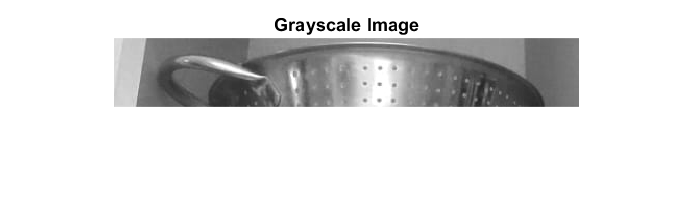
\includegraphics[height=9.5cm, width=\textwidth, keepaspectratio]{Report/Images/Features/Conic/GrayscaleImage.png}
    \caption{\label{fig:conic:gray scale}The image in grey scale}
    \end{figure}

    \item Canny edge detection ($\sigma = 2$, threshold = $[0, 0.15]$)
        \begin{figure}[H]
    \centering
    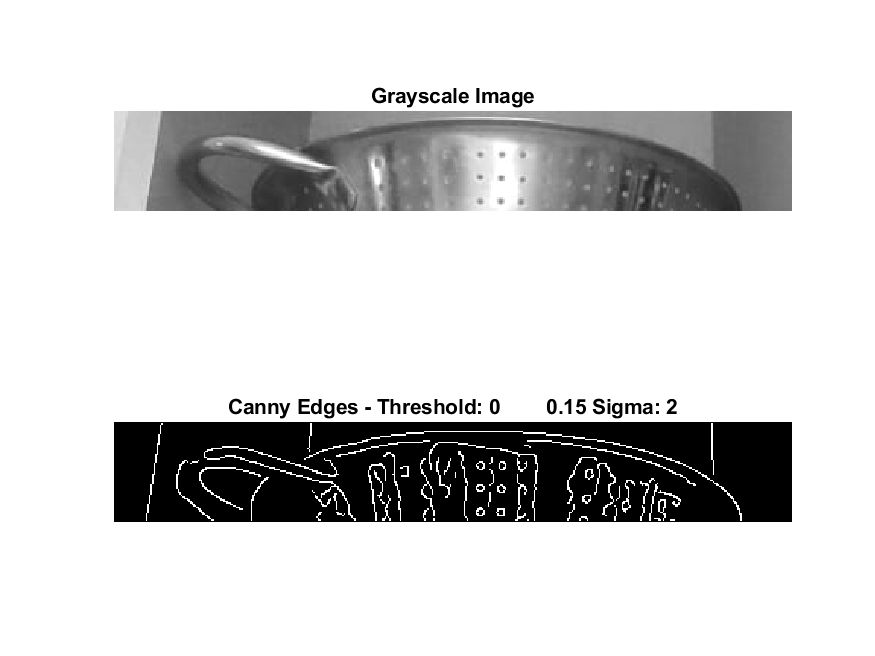
\includegraphics[height=9.5cm, width=\textwidth, keepaspectratio]{Report/Images/Features/Conic/CannyEdges.png}
    \caption{\label{fig:conic:edges}Canny Edge detection}
    \end{figure}

    \item Remove edges that are too crowded, like the holes of the colander. To do that, first heavily blur the image ($\sigma = 10$) then threshold the image to select the sparser areas ($\leq 0.1$). Use this to mask the edges
            \begin{figure}[H]
    \centering
    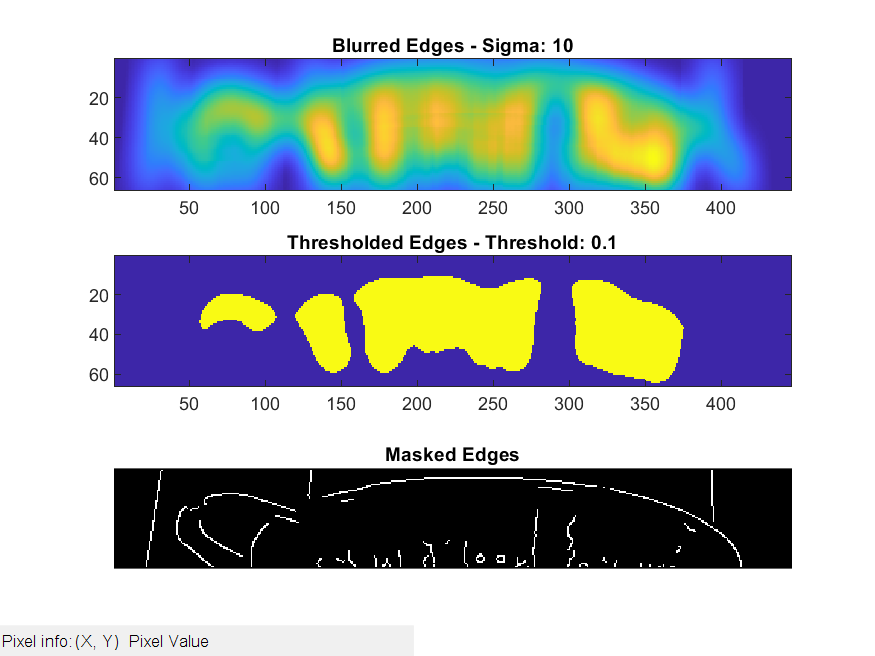
\includegraphics[height=9.5cm, width=\textwidth, keepaspectratio]{Report/Images/Features/Conic/MaskedEdges.png}
    \caption{\label{fig:conic:mask}Masking the edges}
    \end{figure}

    \item Extract the remaining points $\neq 0$ and use a slightly modified RANSAC to extract the Conic with the most inliers 
                \begin{figure}[H]
    \centering
    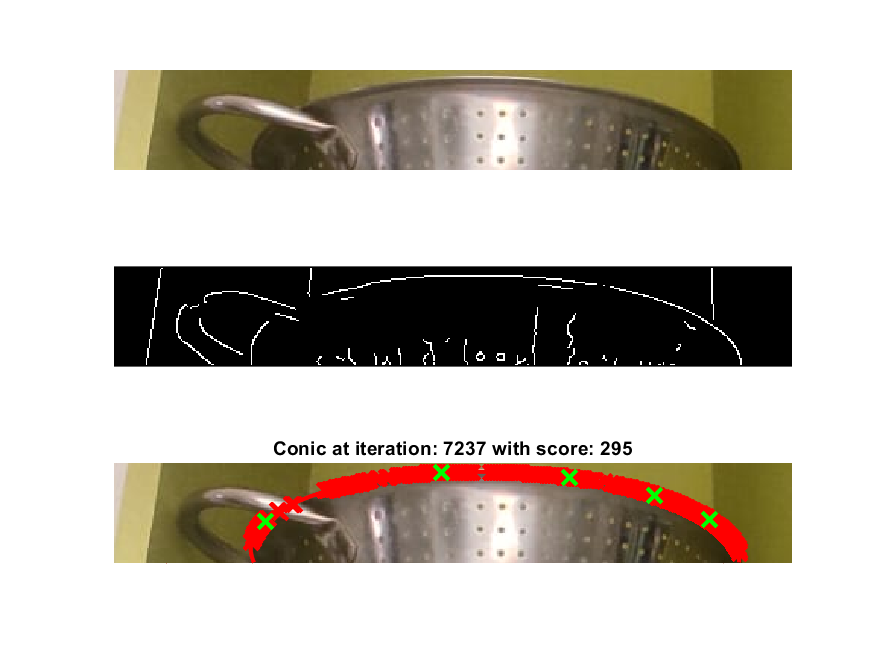
\includegraphics[height=9.5cm, width=\textwidth, keepaspectratio]{Report/Images/Features/Conic/ConicRANSAC.png}
    \caption{\label{fig:conic:ransac}Conic RANSAC}
    \end{figure}

                    \begin{figure}[H]
    \centering
    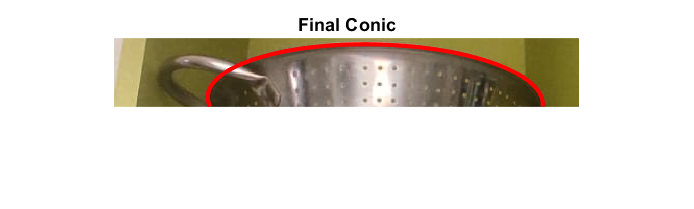
\includegraphics[height=9.5cm, width=\textwidth, keepaspectratio]{Report/Images/Features/Conic/FinalConic.png}
    \caption{\label{fig:conic:final}Final Conic}
    \end{figure}

    
\end{enumerate}

\section{Extraction of $S$ curve}

In order to extract the curve $S$:
\begin{enumerate}
    \item Crop the image to the desired portion
    \item Convert to grayscale
    \item Canny edge detection ($\sigma = 1$, threshold = $[0.2, 0.8]$)
                        \begin{figure}[H]
    \centering
    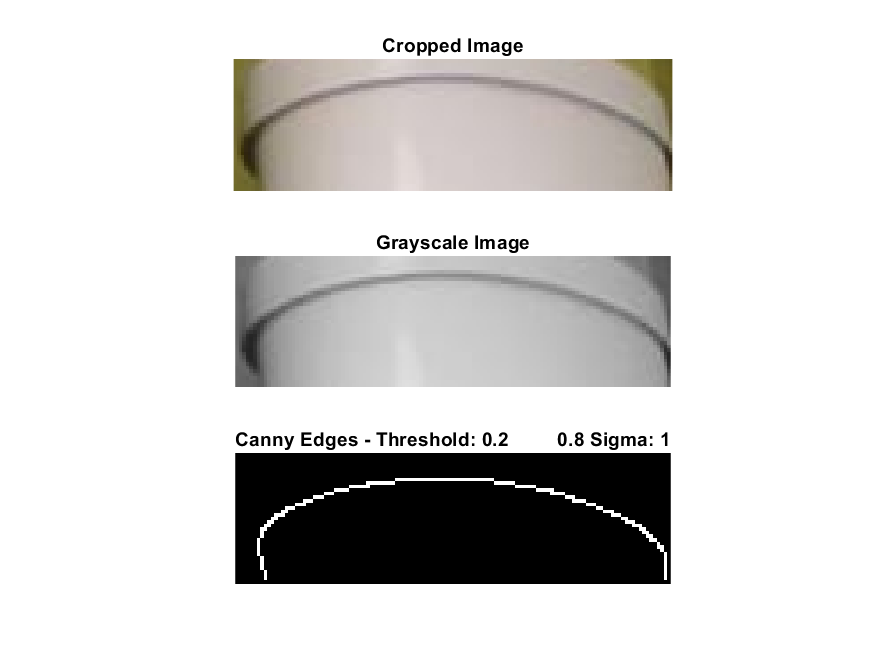
\includegraphics[height=9.5cm, width=\textwidth, keepaspectratio]{Report/Images/Features/S/CannyEdges.png}
    \caption{\label{fig:S extraction}The $S$ extraction process}
    \end{figure}
\end{enumerate}